\newpage
\begin{section}{Arch Linux}
	\begin{subsection}{Mantainance}
		\begin{minted}{sh}
			#check file size
			du -sh .cache/
			#remove a file
			rm -rt .cache/
			#delete what you don't need in .config file
		\end{minted}

		specific mantainance:

		\begin{minted}{sh}
			#check the failed systems
			systemctl --failed
			#check the systemd journal
			sudo journalctl -p 3-xb
			#if the system doesn't boots then ctrl+alt+shift then timeshift -restore
			#then update mirrors
			#clar chache

			#then to update the whole system use:
			sudo pacman -Syyu
			#to check system updates
			sudo pacman -Syu
			#if you wan't to remove all packages in the drive use
			sudo pacman -Scc
			#remove all unwanted dependencies
			paru -Yc 
			#remove orphan packages
			sudo pacman -Rns \$(pacman - Qdtq)
			#sudo pacman -Syyy Syncrhonise data use "mirror1"
		\end{minted}

	\end{subsection}
	\begin{subsection}{Print in arch linux}

		install packages: usbutils, lsusb, cups

		use this to make cups usable
		\begin{minted}{sh}
			sudo systemct enable cups
			sudo systemctl start cups
			localhost:631

			lp -d HP_Officejey_Pro_8600]
		\end{minted}

	\end{subsection}


	\begin{subsection}{configure date and time}

		\begin{minted}{sh}
			hwclock --set --date = "04/32/2021 19:00:00"
			hwclock -hctosys
		\end{minted}

	\end{subsection}

	\begin{subsection}{Configure wireless}

		\begin{minted}{sh}
			#when entering an iso
			iwctl
			#then in the ui

			#to list all available devices
			device list

			#to scan networks
			station <device> scan

			#to get newworks
			station <device> get-network

			#to connect to a network
			station <device> connect "<name of network>"

			#to check if the connection is staable
			ping -c s 8.8.8.8

			#don't forget before rebooting the iso run
			pacman nmtui
		\end{minted}
		from Arch Water Linux
		\begin{minted}{sh}
			# to acces the gui for the internet
			nmtui
			# solve temporary failure in name resolution
			# change the /etc/resolve.conf file to nameserver 8.8.8.8

			# restart the resolved daemon
			sudo systemctl restart systemd-resolved.service
			# check that the daemon is running and active
			sudo systemctl status systemd-resolved.service
		\end{minted}

		dwm basic configuration
		\begin{minted}{sh}
			#MODKEY + shift + q to restart X server
			startx # to start the X server
		\end{minted}

	\end{subsection}
	\begin{subsection}{mount devices}
		mount usb sticks:
		\begin{minted}{sh}
			#to mount a usb stick
			mount /dev/sdb1 /mnt/<destination folder>
			#to unmount a sub stick
			umount /dev/sdb1
		\end{minted}
		mount an android device:
		\begin{minted}{sh}
			#to mount and android device
			simple-mtpfs --device 1 tablet/

			#to unmount an android device
			fusermount -u /tablet

		\end{minted}
	\end{subsection}
	\newpage
	\begin{subsection}{import export passwords from pass}
		export passwords:
		\begin{minted}{sh}
			# to list first the gpg keys
			gpg --list-secret-keys --keyid-format LONG
		\end{minted}
		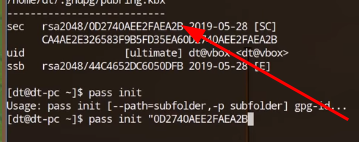
\includegraphics{img_ArchLinux/publicKeyImage.png}
		\begin{minted}{sh}
			# to create the export files
			# save this files in a usb and use it later
			gpg --output MY_FILENAME_public.gpg --armor --export GPG_PUB_KEY
			gpg --output MY_FILENAME_secret.gpg --armor --export-secret-key GPG_PUB_KEY
			# in other pc import the gpg keys
			gpg --import MY_FILENAME_pub.gpg
			gpg --allow-secret-key-import --import MY_FILENAME_sec.gpg
			# now copy the .password-store folder from the main machine and paste it into the new machine
		\end{minted}


	\end{subsection}

	\begin{section}{Install python version}
		\begin{minted}{sh}
	# download the python version you need from https://www.python.org/downloads/source/
	# unpack in the .local/src/pythonversions/pythonVersion.tgz
	tar zxvf pythonVersion.tgz
	cd pythonVersion
	# Install the python version
	./configure
	make
	sudo make install
	make clean
	# check python version
	python[python_version] --version
	# create a python environment using that python version
	python[python_version] -m venv venv/
	# source the environment
	source venv/bin/activate
	# for deactivating
	deactivate
		\end{minted}
	\end{section}

	\begin{subsection}{removing bloatware from android}
	
		\begin{minted}{sh}
		# install the android developer tools
		paru -S android-tools
		# in your android enable developer options by about phone -> build number 7 times
		# then enable usb debugging

		# now in your linux sistem type in your terminal
		adb devices # to see if device is succesfully connected
		adb shell # to start the shell

		# to delete an app
		pm uninstall -k --user -0 (package-name)

		# to see the names of apps use app inspector from the google store
		\end{minted}




\end{subsection}
\begin{subsection}{deploy python django aplication aws}
\begin{minted}{sh}

	## modify the django project

	# settings.py

	STATIC_URL = '/static/'
	STATIC_ROOT = os.path.join(BASE_DIR,'static')

	MEDIA_URL = '/media/'
	MEDIA_ROOT = os.path.join(BASE_DIR,'media')


	## now collect static
	source venv/bin/activate

	python manage.py collectstatic



	### aws
# create an account in aws
# find ec2 and click on launch instance
# select ubunto server 18 free trial
# see all the instances you are running
# change the name of your instance (on the very left side of the row you can do that)
# you will be prompted to create a new id, so create the new keypair and save it to your linux machine
# the right click on the isntance id and click connect
# paste the ssh code in the folder were your keypair is, for example:
ssh -i "password-generator-django.pem" ubuntu@ec2-54-242-121-76.compute-1.amazonaws.com

# now that you are connected sudo update and upgrade the server
sudo apt-get update
sudo apt-get upgrade -y

# you will have to use gnix gnunicorn
python3 --version
python3 -m venv venv/
apt-get install python3-venv
python3 -m venv venv/

ls
# use the environment
source venv/bin/activate

# install django 
pip3 install django


# install necessary packages for python
sudo apt install python3-dev buil-essential 
sudo apt install libssl
sudo aptinstall libssl-dev
sudo apt install libmysqlcient-dev


# install the requirements
pip install -r requirements.txt

# install django-ckeditor
pip3 install django-ckeditor

# git clone your github django project


git clone url.git

cd url

# install modules for deploy
pip3 install gunicorn
sudo apt-get install -y nginx

# start nginx
sudo nginx

# configure security groups in for https and http
right click(on the instance row) -> networking -> change security group -> see the launch wizar asociated with the instance

click security groups -> launch wizard n -> inbound -> edit -> add rule 

\end{minted}

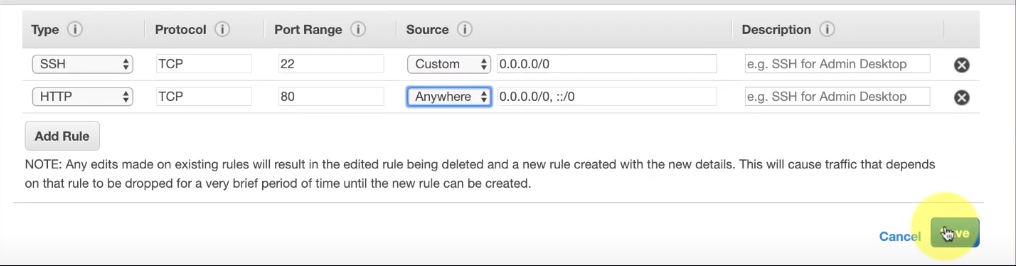
\includegraphics{img_ArchLinux/inboundRules.png}
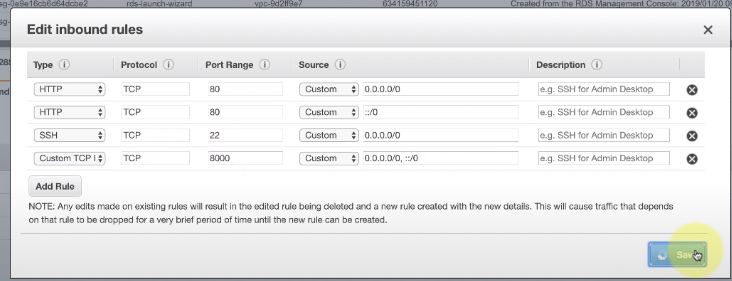
\includegraphics{img_ArchLinux/inboudUpdate.png}

\begin{minted}{sh}
# to connect the gunicorn (which is the wsgi interface 
# tell gunicorn to use the wsgi.py
cd project/project
gunicorn --bind 0.0.0.0:8000 project.wsgi:application
# after this you sould be able to acces your web app using the link
# use the port 8000 example: google.com:8000

# supervisor makes sure your application is running always
sudo pat-get install -y supervisor
# create a configuration for supervisor
cd /etc/supervisor/conf.d/
touch gunicorn.conf
sudo touch gunicorn.conf

# edit it
sudo nvim gunicorn.conf

# inside the file
[program:gunicorn]
directory=/home/ubuntu/project
command=/home/ubuntu/env/bin/gunicorn --workers 3 --bind unix:/home/ubuntu/project/app.sock 
	testproject.wsgi:application

autostart=true
autorestart=true
stderr_logfile=/var/log/gunicorn.err.log
stdout_logfile=/var/log/gunicorn.out.log

[group:guni]
programs:gunicorn

# save and exti
# outside the file
sudo mkdir /var/log/gunicorn
sudo supervisorctl reread

sudo supervisorctl update

sudo supervisorctl status 

# nginx configuration
cd ~
cd /etc/nginx/sites-available
sudo touch django.conf
sudo nvim django.conf

# paste the code

	server{
		listen 80;
		server_name ec2-3-91-188-252.compute-1.amazonaws.com;
		location / {
			include proxy_params;
			proxy_pass http://unix:/home/ubuntu/personal_portfolio/app.sock;
		}
		location /static/ {
			autoindex on;
			alias /home/ubuntu/personal_portfolio/static/;
		}
		location /media/ {
			root /home/ubuntu/personal_portfolio/;
		}
		}


# save and exit
sudo nginx -t

# enable the link
sudo ln django.conf /etc/nginx/sites-enabled/


# save and exit
sudo nginx -t

sudo service nginx restart








######
## now for setting static files
#####

# in settings.py
STATIC_URL = '/static/'

# in the html you are doing


# in the templates section
'DIRS':[os.path.join(BASE_DIR,'TestProject/templates')],

# open the server with the keys and cd 
nvim /etc/nginx/sites-enabled/django.conf

# append

location /static/ {
	autoindex on;
	alias /home/ubuntu/ProjectFolder/MainProjectFolder/static/;
}

# outside the file
# open the nginx configuration to allow big pictures

cd /etc/nginx
sudo vim nginx.conf

#inside the http or server paste
client_max_body_size 4M;



sudo systemctl reload nginx ;












######
## now for setup the database with django
#####


# create database
dtaabase section ->
RDS ->
create database ->
mysql ->
only enable options eligible for free usage ->
next ->
select the specific mysql version ->
database instance offered on the free tier ->
allocated storage
configure the name,username,password etc
allow public accesibility
choose default existing vpc security groups
database name

# now get the latest code in your github
git pull
# configure the database for the server
DATABASES = {
	# name
	'default' : {
		'ENGINE':"django.db.backends.mysql",
		'NAME':"database_name",
		'USER':"database_user",
		# change this manually in the server
		"PASSWORD":"********",
		# click on the database, check endpoint & port for configuring
		'HOST','host',
		'PORT':'12312'
	}
}
# activate the environment
source venv/bin/activate

# install all the modules in the requirements
pip install django-mysql

# make the migrations
python manage.py makemigrations name_of_main_app
python manage.py migrate

# reestart the server
sudo supervisorctl reload

sudo service nginx restart
\end{minted}
\end{subsection}


\begin{subsection}{use nvim for graphical programs}
	\begin{minted}{sh}
		# first you have to make it the default
		# in .zshrc put
		VISUAL=nvim
		EDITOR=nvim

		# then change the nvim.desktop in /usr/share/applications/nvim.desktop
		and place 
		EXEC=nvimWrapper
		TRY=nvimWrapper %F

		# now create the wrapper in the bin like
		st -e sh -c "nvim \$1"
	\end{minted}
\end{subsection}
\end{section}


